Quelltexte können in zwei verschiedenen Kontexten in Fragestellungen auftauchen: Einerseits gibt es unvollständige, kurze Quelltext-Fragmente, die in einen Fließtext eingebunden werden sollen, wie in diesem Beispiel:

\begin{center}
„Wie viele String-Parameter hat die folgende Java-Methode?\newline
public String m(int i, int s, boolean b) \{ ... \}“
\end{center}

Dabei handelt es sich nicht um ein syntaktisch nicht vollständiges und nicht-ausführbares Java-Fragment. Um die Lesbarkeit dieses Fragments zu erhöhen, sollte es trotzdem optisch deutlich vom Fließtext unterscheidbar sein. Es bietet sich an, den Code in einer Monospace-Schriftart zu formatieren und (wenn möglich) eine syntaktische Einfärbung (Syntax Highlighting) anzuwenden.

Da die Entwicklung einer eigenen Editor-Komponente extrem komplex ist, und es in diesem Bereich bereits eine große Auswahl an Bibliotheken gibt, wird auch hier auf eine bestehende Implementierung zurückgegriffen. Dabei müssen folgende Anforderungen von einer solchen Bibliothek erfüllt werden:

\begin{itemize}
    \item \textbf{Integration in React:}  Muss sich leicht in das deklarative React-Framework einbinden lassen.
    \item \textbf{WYSIWYG (What You See Is What You Get):} Der Editor sollte stets eine Vorschau aller Formatierungen darstellen, und man sollte nicht zwischen einem Markup- und einem Vorschau-Modus wechseln müssen. Formatierungen sollen über Buttons eingefügt werden können.
    \item \textbf{Text-Formatierungen:} Der Editor muss über simple Text-Formatierungen verfügen (zum Beispiel Fettschrift und Kursivierung).
    \item \textbf{Monospace-Schriftart:} Eine Möglichkeit zum Verwenden einer Monospace-Schriftart muss vorhanden sein.
    \item \textbf{Syntax Highlighting:} Syntax-Highlighting von Code-Fragmenten muss unterstützt werden (üblicherweise durch ein Plugin/Erweiterung mit einer zusätzlichen Bibliothek wie Highlight.js).
\end{itemize}

Nach dem Erwägen und Ausprobieren diverser Bibliotheken (zum Beispiel Draft.js, Slate, Prosemirror, Quill) fiel die Wahl letztendlich auf den Quill-Editor\cite{web:quill}, der alle genannten Anforderungen erfüllt. Quill ist nicht primär für den Einsatz mit React vorgesehen, deswegen wurde diese Bibliothek in Form einer Wrapper-Bibliothek, die Quill in React-Komponenten bündelt, verwendet. Leider ist diese \texttt{react-quill}-Bibliothek\cite{web:react_quill} nicht sehr gut gepflegt und nicht auf dem neusten Stand in Bezug auf die eingesetzte Editor-Version, so dass sie einige Fehler mitbringt.

\begin{figure}[H]
    \centering
    \setlength{\fboxsep}{0pt}
    \setlength{\fboxrule}{0.5pt}
    \fbox{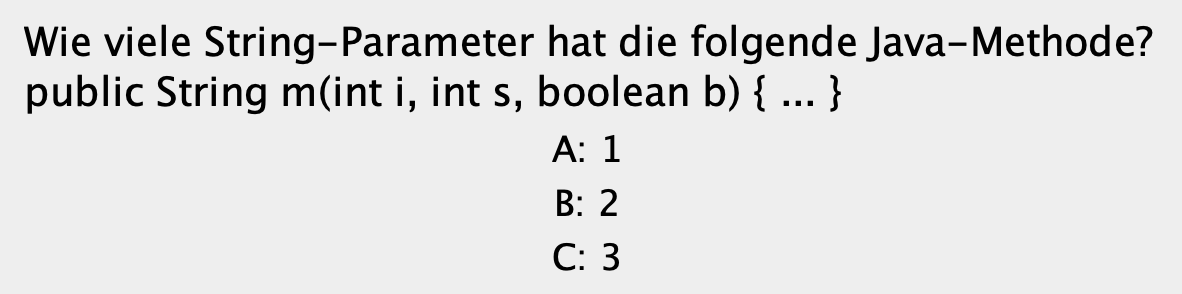
\includegraphics[width=\textwidth-1pt]{chapter/entwurf/bilder/sturesy_fragment.png}}
    \caption{Darstellung eines Code-Fragments in StuReSy (ohne manuell vorgenommene  Formatierungen)}
    \label{abb:sturesy_code_fragment}
\end{figure}


\begin{figure}[H]
    \centering
    \setlength{\fboxsep}{0pt}
    \setlength{\fboxrule}{0.5pt}
    \fbox{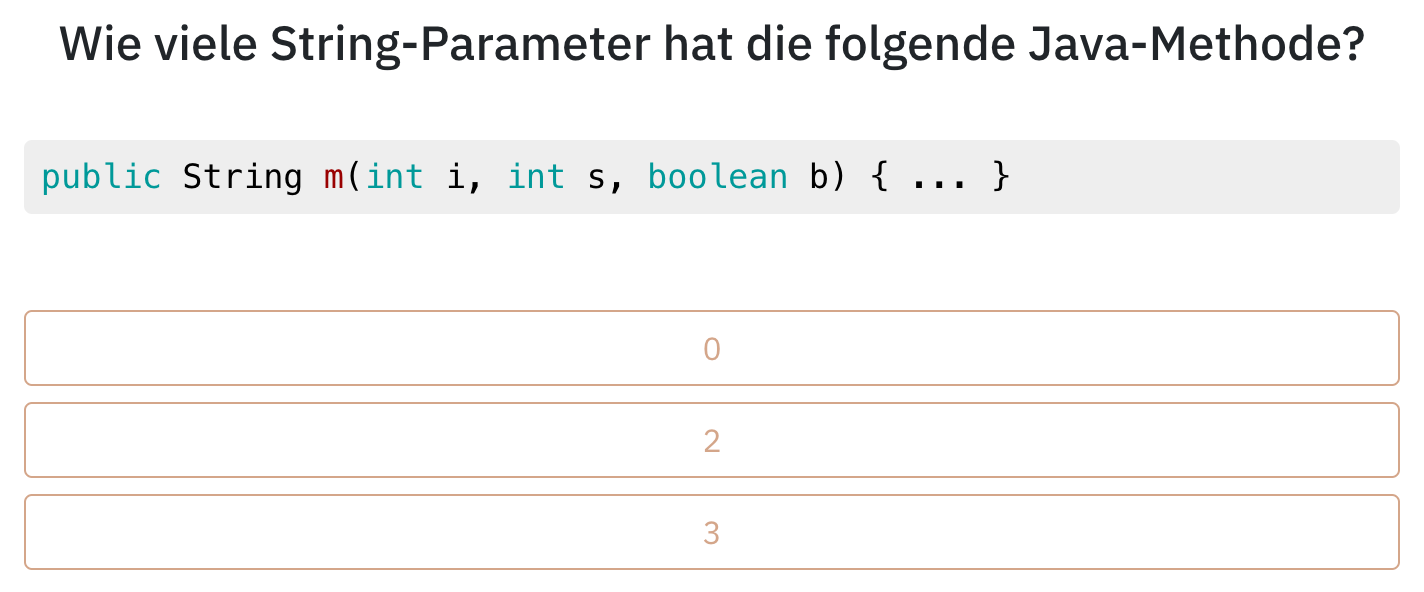
\includegraphics[width=\textwidth-1pt]{chapter/entwurf/bilder/weclare_fragment.png}}%
    \caption{Darstellung eines Code-Fragments in Weclare (Quelltext als Code-Block ausgezeichnet)}
    \label{abb:weclare_code_fragment}
\end{figure}

Der zweite Kontext von Quelltexten in Fragestellungen ist das Einfügen von vollständigem, ausführbarem Code, zum Beispiel in Form ganzer Klassen. Solcher Code kann in Weclare direkt im Browser ausgeführt werden. Ein solches, interaktives Code-Beispiel kann allerdings nur einmal pro Frage vorhanden sein und ist auch nicht Teil des Fließtexts. Eine entsprechende Editor-Komponente zum Einfügen solchen Codes sollte also auch funktional darauf zugeschnitten sein: Text-Formatierungen sind nicht mehr notwendig, stattdessen rücken Funktionen wie die korrekte Einrückung von Code-Zeilen und Zeilen-Nummerierungen in den Vordergrund.

Der Quill-Editor kann leider nicht in einem „Code only“-Modus betrieben werden, so dass eine zweite, unabhängige Editor-Komponente für interaktive Code-Abschnitte integriert wird. Mit CodeMirror\cite{web:codemirror} gibt es eine sehr beliebte Bibliothek für diesen Zweck, die allerdings auch nicht explizit für den Einsatz mit React bestimmt ist, so dass auch sie in Form einer Wrapper-Bibliothek namens \texttt{react-codemirror2}\cite{web:react_codemirror2} zum Einsatz kommt.

\begin{figure}[H]
    \centering
    \setlength{\fboxsep}{0pt}
    \setlength{\fboxrule}{0.5pt}
    \fbox{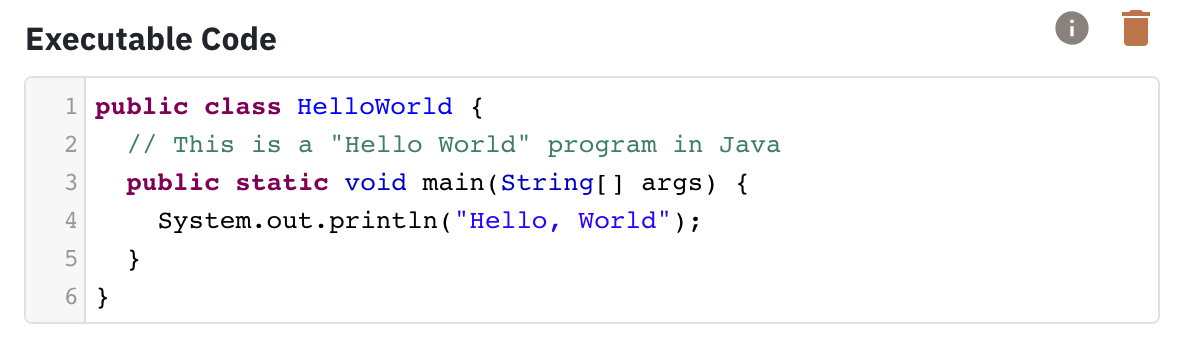
\includegraphics[width=\textwidth-1pt]{chapter/entwurf/bilder/weclare_codemirror.png}}
    \caption{Darstellung eines ausführbaren Java-Quelltexts in Weclare mittels der CodeMirror-Bibliothek.}
    \label{abb:weclare_codemirror}
\end{figure}